%============================================================%
\documentclass[a4paper,12pt]{article}
%%%%%%%%%%%%%%%%%%%%%%%%%%%%%%%%%%%%%%%%%%%%%%%%%%%%%%%%%%%%%%%%%%%%%%%%%%%%%%%%%%%%%%%%%%%%%%%%%%%%%%%%%%%%%%%%%%%%%%%%%%%%%%%%%%%%%%%%%%%%%%%%%%%%%%%%%%%%%%%%%%%%%%%%%%%%%%%%%%%%%%%%%%%%%%%%%%%%%%%%%%%%%%%%%%%%%%%%%%%%%%%%%%%%%%%%%%%%%%%%%%%%%%%%%%%%
\usepackage{eurosym}
\usepackage{vmargin}
\usepackage{amsmath}
\usepackage{graphics}
\usepackage{epsfig}
\usepackage{subfigure}
\usepackage{multicol}
\usepackage{fancyhdr}
\usepackage{listings}
\usepackage{framed}
\usepackage{graphicx}
\usepackage{amsmath}
\usepackage{enumerate}
\usepackage{chngpage}
%\usepackage{bigints}


\setcounter{MaxMatrixCols}{10}

\begin{document}
	\begin{center}
		
\includegraphics[scale=0.55]{images/shieldtransparent2}
	\end{center}
	
	\begin{center}
		\vspace{1cm}
		\large \bf {FACULTY OF SCIENCE AND ENGINEERING} \\[0.5cm]
		\normalsize DEPARTMENT OF MATHEMATICS AND STATISTICS \\[1.25cm]
		\large \bf {REPEAT EXAMINATION PAPER 2017} \\[1.5cm]
	\end{center}
	
	\begin{tabular}{ll}
		MODULE CODE: MA4605 & SEMESTER: Repeat 2017 \\[1cm]
		MODULE TITLE: Chemometrics & DURATION OF EXAM: 2.5 hours  \\
		 & \\ [1cm]
		LECTURER: Mr. Kevin O'Brien & GRADING SCHEME: 100 marks \\
		& \phantom{GRADING SCHEME:} \footnotesize {60\% of module grade} \\[1cm]
EXTERNAL EXAMINER: Prof. A. Marshall & \\
	\end{tabular}
\vspace{0.3cm}
	\begin{center}
		{\bf INSTRUCTIONS TO CANDIDATES}
	\end{center}
	
	{\noindent \\ Scientific calculators approved by the University of Limerick can be used. \\
		Formula sheet and statistical tables provided at the end of the exam paper.\\
		There are 5 questions in this exam. Students must attempt any 4 questions.}
	%====================================================================== %
	\newpage
\bigskip
%--------------------------------------------------------------------------------------- %

\subsection*{Question 1. (25 marks) Inference Procedures}
	
\begin{itemize}

\item[(a)]

%\subsubsection*{Part A : Outliers}
\begin{itemize}
	\item[(i.)] (3 Marks) Provide a brief description for three tests from the family of Grubb's  Outliers Tests. Include in your description a statement of the null and alternative hypothesis for each test
	\item[(ii.)] (2 Marks) Describe any required assumptions for tests, and the limitations of these tests.
\end{itemize}



% Review of Univariate Normal Distribution
% Test for Univariate normality
% - Graphical Procedures
% - Formal Tests
% (Later Multivariate Normality)
% Boxplots, Outliers and Transformations
%
% (Hint: there are no outliers in these data sets)

\item[(b)]
Numeric Transformations, such as logarithmic transformation, are often used in statistical analysis as an approach for dealing with non-normal data.
\begin{itemize}
	\item[(i)] (1 Marks) Discuss the importance of numeric transformations, such as logarithmic transformation, in Statistics.
	%	\item[(ii)] Describe the process of transformations
	%	\item[(i.)] (1 Mark) Describe the purpose of Tukey's Ladder (referencing direction and relative strength).
	\item[(ii.)] (3 Marks) Give two examples of a transformation for various types of skewed data (i.e. an example for both types of skewness).
	\item[(iii.)] (1 Mark) Discuss the limitations of numeric transformations.
\end{itemize}

	\item[(c)]
Consider the following inference procedure performed on data set $Z$.
\begin{center}
	\begin{framed}
		\begin{verbatim}
		> shapiro.test(Z)
		
		Shapiro-Wilk normality test
		
		data:  Z
		W = 0.8914, p-value = 0.007047
		
		\end{verbatim}
	\end{framed}
\end{center}


\begin{itemize}
	\item[(i.)] (1 Mark) Describe what is the purpose of this procedure.
	\item[(ii.)] (1 Mark) What is the null and alternative hypothesis?
	\item[(iii.)] (1 Mark) Write the conclusion that follows from it.
	\item[iv.] (1 Mark) Tests for Normality are known to be susceptible to low power. Discuss what is meant by this.
\end{itemize}


	\item[(d)] A graphical procedure was carried out to assess whether or not this assumption of normality is valid for data set \texttt{Z}. Consider the figure below.

\begin{center}
	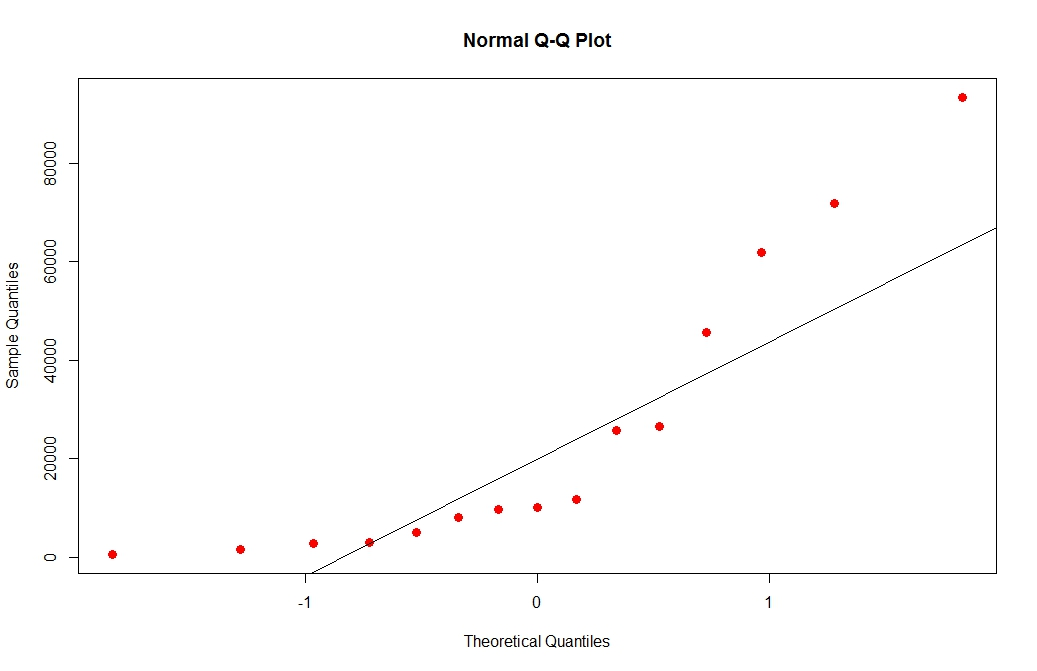
\includegraphics[scale=0.40]{images/MT2016-QQPLOT}
\end{center}

\begin{itemize}
	\item[(iv.)] (1 Mark) Provide a brief description on how to interpret this plot.
	\item[(v.)] (1 Mark) What is your conclusion for this procedure? Justify your answer.
\end{itemize}



\item[(e)] (5 Marks)

A test of a specific blood factor has been devised such that, for adults in Western Europe, the test score is normally distributed with mean 100 and standard deviation 10. A clinical research organization is carrying out research on the blood factor levels for individuals with a particular disease, with emphasis on the effects of medication on the blood factor level.

For a group of 10 volunteer patients the following test scores were obtained both prior to, and after the medication.

\begin{center}
\begin{tabular}{|c||c|c|c|c|c|c|c|c|c|c|} \hline 
Patient	& A	& B	& C	& D	& E	& F	& G &	H &	I &	J	\\ \hline  \hline
Before	& 120& 	140	& 112 &	109&	114	& 116 &	99 & 	108 &	109	& 111 \\ \hline 	
After	& 104&	112	& 110 &	107&	101	& 103 &	101	& 102&	103	& 102 \\ \hline 
\end{tabular} 
\end{center}
	


The organization wishes to determine if there is a significant improvement (lessening of the blood factor level) due to the medication.  Using the output, shown below, write a short report discussing your findings. State the null and alternative hypotheses clearly. (You may assume that the case-wise differences are normally distributed.)
\textit{(The \texttt{R} output is presented on the next page)}
\newpage

\begin{framed}
\begin{verbatim}
> t.test(Before,After,paired=TRUE)

Paired t-test

data:  Before and After
t = 3.3881, df = 9, p-value = 0.008023
alternative hypothesis: 
  true difference in means is not equal to 0
  
95 percent confidence interval:
3.090618 15.509382
sample estimates:
mean of the differences 
9.3 
\end{verbatim}
\end{framed}
\bigskip

\item[(f)] (5 Marks)
The research organization wishes to assess the link between the blood factor level and intake of a particular supplement.  Using the following output, write a short report discussing your findings. State the null and alternative hypotheses clearly.



\begin{framed}
\begin{verbatim}
> cor.test(BloodFactor,Supplement)

Pearson's product-moment correlation

data:  BloodFactor and Supplement
t = -1.384, df = 13, p-value = 0.1896
alternative hypothesis: true correlation is not equal to 0
95 percent confidence interval:
-0.7355908  0.1885016
sample estimates:
cor 
-0.3583659 

> 

\end{verbatim}
\end{framed}
\end{itemize}


%--------------------------------------------------------------------------------------------------------%

\newpage



\subsection*{Question 2. (25 marks) Regression Models }
	% Multiple Linear Regression
\begin{itemize}


\item[(a)] 


The fluorescence of each of a series of acidic solutions of quinine with concentrations 0,10,20,30,40,50 and 60
was determined five times. The mean values and standard deviations of these determinations have
been obtained as follows:
\begin{center}
	\begin{tabular}{|c|ccccccc|}
		\hline
		% after \\: \hline or \cline{col1-col2} \cline{col3-col4} ...
		Means: & 4.0 & 21.2& 44.6& 61.8& 78.0 &105.2&121.6\\
		Std Deviations: &0.71& 0.84 &0.89 &1.64 &2.24 &3.03&4.05\\
		\hline
	\end{tabular}
\end{center}


\begin{figure}[h!]
	\centering
	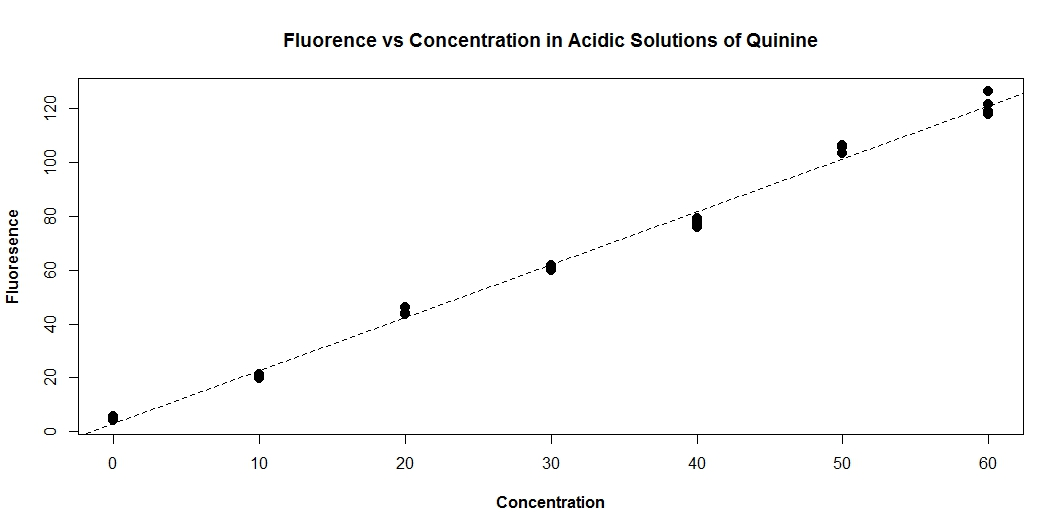
\includegraphics[width=0.7\linewidth]{images/Q2-Quinine}
	\caption{}
	\label{fig:Q2-Quinine}
\end{figure}

The model is described by the following \texttt{R} code output. Another code segment in on the top of the next page. Answer the questions on the next page.


\begin{framed}
	\begin{verbatim}
		> summary(lm(Fluo~Conc))
		
		Call:
		lm(formula = Fluo ~ Conc)
		
		Residuals:
		    Min      1Q  Median      3Q     Max 
		-5.9645 -2.1473  0.2626  1.9254  5.2553 
		
		Coefficients:
		            Estimate Std. Error t value Pr(>|t|)    
		(Intercept)  2.95221    1.01033   2.922  0.00711 ** 
		Conc         1.96844    0.02802  70.247  < 2e-16 ***
		---
		Signif. codes:  0 ‘***’ 0.001 ‘**’ 0.01 ‘*’ 0.05 ‘.’ 0.1 ‘ ’ 1
		
		Residual standard error: 2.966 on 26 degrees of freedom
		Multiple R-squared:  0.9948,    Adjusted R-squared:  0.9946 
		F-statistic:  4935 on 1 and 26 DF,  p-value: < 2.2e-16

		
		\end{verbatim}
	\end{framed}
\newpage
\begin{framed}
\begin{verbatim}			

		> confint(lm(Fluo~Conc))
		                 2.5 %   97.5 %
		 (Intercept) 0.8754463 5.028968
		 Conc        1.9108368 2.026035
	\end{verbatim}
\end{framed}


\begin{enumerate}[(i)]
	\item (3 marks)
	What is the regression equation for this fitted model? In your answer, Interpret the slope and the intercept of the regression line.
	\item (3 Marks) Comment on the significance of the regression estimates.
	\item (2 Marks) State the 95\% confidence interval for the slope and the intercept coefficients. Interpret this intervals with respect to any relevant hypothesis tests

	\item (2 Marks) Explain in which way is the prediction intervals different from the confidence intervals for fitted values in linear regression?
\end{enumerate}


\item[(b)] Model appraisal and validation are importants steps in the statistical modelling process. Answer the following questions.
\begin{itemize}
	\item[(i)] (2 Marks) In the context of regression models, explain what is meant by Heteroscedascity and Homoscedascity. Support your answers with sketches.
	
	
	\item[(ii)] (1 Mark)  Explain how the \emph{Akaike information criterion} would used to compare two models fitted for the same data.
	
	\item[(iii)] (1 Mark) Explain why the adjusted $R^2$ value may differ in value from the corresponding multiple $R^2$ value for the same fitted model.
	
	
	\item[(iv)] (1 Marks) Explain the term ``Influence" in the context of linear regression models. Support your answer with sketches.
	\item[(v)] (1 Marks) Explain the  term ``Cook's Distance" in the context of linear regression models. 
	
	
	
	\item[(vi)] (2 Marks)  The Durbin Watson Test was carried out to test for Autocorrelation. Briefly describe autocorrelation. You may support your answer with sketches.
	\item[(vii)] (1 Mark) State your conclusion to the following procedure.
	\begin{framed}
		\begin{verbatim}
		> durbinWatsonTest(myModel)
		lag Autocorrelation D-W Statistic p-value
		1     -0.08428163      2.143578   0.806
		Alternative hypothesis: rho != 0
		\end{verbatim}
	\end{framed}
\newpage
\end{itemize}
\item[(c)] (6 Marks) Suppose we have a regression model, described by the following equation
\[ \hat{y} = 18.81 + 6.25x_1 + 7.82 x_2 - 1.74 x_3\]
We are given the following pieces of information.
\begin{itemize}
\item[$\ast$] The standard deviation of the response variance $y$ is 10 units.
\item[$\ast$] There are 76 observations.
\item[$\ast$] The \textit{Coefficient of Determination} (also known as the \textit{Multiple R-Squared}) is 0.80.
\end{itemize}
Complete the \textit{Analysis of Variance} Table for a linear regression model.
The required values are indicated by question marks.

\begin{center}
	\begin{tabular}{|c|c|c|c|c|c|} \hline
		\phantom{makespace}	& DF & 	Sum Sq &	Mean Sq &	F value &   	Pr($>$F)    \\ \hline
		Regression &  \phantom{make}?\phantom{make} &	? &	? &	 ? &	$< 2.2e^{-16}$ \\ \hline
		Error  & ? &	? &  	?   &            &       \\ \hline
		Total  & ?  &	? &  \phantom{makespace}	  &   \phantom{makespace}         &    \phantom{makespace}    \\ \hline
	\end{tabular} 
\end{center}






\end{itemize}
\bigskip

\subsection*{Question 3. (25 marks) Experimental Design }
\begin{itemize}
	\item [(a)]

Specimens of milk from dairies in four different districts are assayed for their concentrations of the radioactive isotope Strontium-90. 
The results, in picocuries per litre, are shown in the table below.


	\begin{center}
		\begin{tabular}{|c|cccccccc|c|c|}
			\hline  

	 & &&&&&&& & Mean & St. Dev \\  
		District	&  &&&&&&&& $\bar{x}_i$ & $s_{i}$ \\  
		\hline \hline
A&	28.2	&	30.8	&	27.8	&	32.7	&	29.6	&	31.3	&	32.4	&	32.8	&	30.7	&	1.855	\\ \hline
B&	30.3	&	28.5	&	32.4	&	31.6	&	28.6	&	34.6	&	31.6	&	31.2	&	31.1	&	1.874	\\ \hline
C&	32.9	&	30.6	&	33.6	&	37.1	&	32.6	&	36.1	&	35.5	&	34.4	&	34.1	&	1.976	\\ \hline
D&	32.8	&	34.8	&	34	&	31.6	&	34.8	&	35.2	&	36.4	&	39.6	&	34.9	&	2.251	\\ \hline \hline
			Overall & &&&&&&&&	32.7	&	2.660	\\ \hline
		\end{tabular} 
	\end{center}


%\bigskip
%\begin{itemize}
%	\item[(i)] (2 Marks) Showing your workings, compute the \textbf{Between Group Sum of Squares} (\textit{SSbetween}).
%	\item[(ii)] (2 Marks) Showing your workings, compute the \textbf{Within Group Sum of Squares}\\ (\textit{SSwithin}).
%	\item[(iii)] (2 Mark) Showing your workings, compute the \textbf{Total Group Sum of Squares} (\textit{SStotal}).
%	\item[(iv)] (1 Mark) Complete the \textbf{Degrees of Freedom} Column for the ANOVA table below.
%	\item[(iv)] (1 Mark) Complete the \textbf{Mean Square} Column for the ANOVA table below.
%	\item[(iv)] (1 Mark) Complete the \textbf{F} Column (i.e. the column for Test Statistic) for the ANOVA table below.
%\end{itemize}

%The following \texttt{R} output has been produced as a result of analysis of these data:

%Experiment=data.frame(Determinations, Analyst)
%Model=aov(Determinations~Analyst)
%summary(Model)

%Analysis of Variance Table
%
%            Df Sum Sq Mean Sq F value  Pr(>F)
%Analyst      5 0.8611 0.17222   4.236 0.00394 **
%Residuals   36 1.4635 0.04065
%---
%Signif. codes:  0 ‘***’ 0.001 ‘**’ 0.01 ‘*’ 0.05 ‘.’ 0.1 ‘ ’ 1


\begin{enumerate}[(i)]
	\item (8 Marks) Complete the ANOVA table in your answer sheet, replacing the ``?" entries with the correct values.
	\item (1 Mark) What hypothesis is being considered by this procedure.
	\item (1 Mark) What is the conclusion following from the above analysis? State the null and alternative hypothesis clearly.
	\item (2 marks) State any two assumptions underlying the ANOVA model?
\end{enumerate}

\bigskip
{
	
	\begin{center}
		\begin{tabular}{|l||c|c|c|c|}
			\hline \phantom{makespace} & DF & SS & MS & F \\ \hline
			\hline Between & \phantom{make}? \phantom{make} & \phantom{make}? \phantom{make} & ?  &  ?\\ 
			\hline Within & \phantom{make}? \phantom{make} &\phantom{make}? \phantom{make}  &\phantom{make}? \phantom{make} &  \\ \hline
			\hline Total &  \phantom{make}? \phantom{make} &  &\phantom{makespace}  & \phantom{makespace} \\ 
			\hline 
		\end{tabular} 
	\end{center}
}
\bigskip

\item[(b)] (4 Marks) The following outputs are Post-Hoc Procedures for the example in part (a). Interpret these outputs.

\begin{framed}
	\begin{verbatim}
	Tukey Pairwise Comparisons 
	
	Grouping Information Using the Tukey Method and 95% Confidence
	
	District  N    Mean  Grouping
	D         8  34.900  A
	C         8  34.100  A
	B         8  31.100    B
	A         8  30.700    B
	
	\end{verbatim}
\end{framed}

	
	\begin{figure}[h!]
\centering
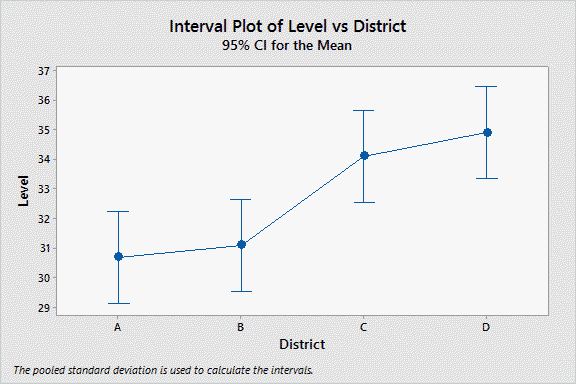
\includegraphics[width=0.85\linewidth]{images/PostHoc1}
\end{figure}
\textit{(The computer output continues on the next page.)}
\newpage
	\begin{figure}[h!]
		\centering

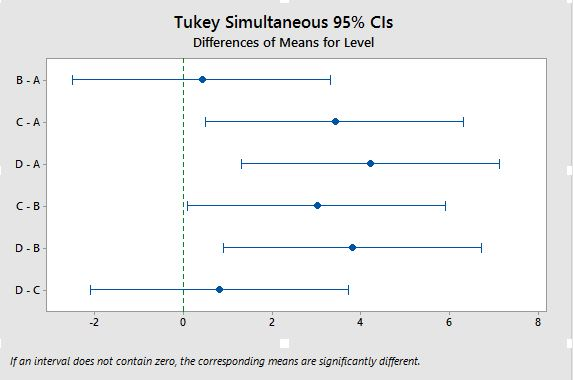
\includegraphics[width=0.85\linewidth]{images/PostHoc4}

\end{figure}

\item[(c)] 
Five standard solutions of chloride were prepared. Four titration methods, each with a different technique of end-point determination, were 
used to analyze each standard solution. The order of the experiments was randomized. The results of chloride found are shown below.


\begin{table}[ht]
	\centering
	\begin{tabular}{|r||c|c|c|c|}
		\hline
		& Method U & Method V & Method W & Method X \\ 
		\hline
	Solution 1 & 10.15 & 10.64 & 10.71 & 10.71 \\ 
	Solution 2 & 10.13 & 10.23 & 10.72 & 10.01 \\ 
	Solution 3 & 10.32 & 10.22 & 10.60 & 10.24 \\ 
	Solution 4 & 10.29 & 10.72 & 10.53 & 10.58 \\ 
	Solution 5 & 9.81 & 10.28 & 10.20 & 9.99 \\ 
		\hline
	\end{tabular}
\end{table}


%\begin{enumerate}[(i)]
%%	\item In the context of the above example, distinguish between the treatment and the blocking variables involved. Give reasons.
%%	
%%	
%%	
%%	\item The above data are an example of a particular experimental design. What is the general name given to this type of experimental design? Name one serious limitation of this type of experimental design.
%%	
%	
%	
%	\item Complete the ANOVA table substituting the symbols ? with their correct values.
%	
%	
%	
%	\item Interpret the results.
%	
%	
%	
%	\item What is the key property of the experimental design above which allows factor effects to be estimated independently of one another. Show how this property presents itself in the above design.
%	
%	
%\end{enumerate}
	
	\noindent You are also given the following information:
	\begin{itemize}
		\item[$\bullet$] $S^2_r = 0.0394$
		\item[$\bullet$] $S^2_c = 0.0305$
		\item[$\bullet$] The variance of concentrations in the table above is $\mbox{Var}(y) = 0.0771$
	\end{itemize}

	\noindent The following questions will result in the completion of the ANOVA Table on the next page. The $p-$values for both tests are already provided.
	\begin{itemize}
		\item[(i)](7 Marks) Complete the ANOVA Table. Show your workings.

		\item[(ii)] (2 Marks) Based on the p-values, provided, what is your conclusion? Clearly state the null and alternative hypotheses for both tests.
	\end{itemize}
	
	\begin{center}
		\begin{tabular}{|c||c|c|c|c|l|}
			\hline Source & DF & SS & MS & F & p-value \\ \hline 
		 Factor A & \phantom{mak} ? \phantom{mak}  & \phantom{mak} ? \phantom{mak}  & \phantom{mak} ? \phantom{mak}  & \phantom{mak} ? \phantom{mak}  &0.0130 * \\ 
			\hline Factor B & \phantom{mak} ? \phantom{mak}  & \phantom{mak} ? \phantom{mak}  & \phantom{mak} ? \phantom{mak}  & \phantom{mak} ? \phantom{mak}  & 0.0196 *    \\ \hline
		Error &  ? & ? & \phantom{mak} ? \phantom{mak}  &  &  \\ 
			\hline \hline Total & ? & ? &  &  &  \\ 
			\hline 
		\end{tabular}
	\end{center} 





\end{itemize}
\normalsize{
	
\newpage	

\section*{Question 4. (25 Marks) Experimental Design}
\begin{itemize}
	\item[(a)]
	
	\begin{enumerate}[(i)]
		%-----------------------%
	%	\item (2 Marks) What is the purpose of a post hoc test?
	%	\item (3 Marks) What are the key components that need to be identified when designing an experiment?
		
		\item (2 Marks) What is a randomised block design?
		\item (2 Marks) What is an ``a x b" factorial experimental design?
		\item (2 Marks)  What is the difference between a between-treatments estimate and a within treatments estimate?
		\item (2 Marks) What distinguishes a factorial experiment from a completely randomised experiment or a randomised block experiment?
		
		
	\end{enumerate}


		\item[(b)] 
		An experiment is run on an operating chemical process in which the aim is to reduce the
		amount of impurity produced. Three continuous variables are thought to affect impurity,
		these are concentration of NaOH, agitation speed and temperature. As an initial investigation two settings are selected for each variable these are
		
\begin{center}
	\begin{tabular}{|c|c|c|}
		\hline
		% after \\: \hline or \cline{col1-col2} \cline{col3-col4} ...
		Factor: &low level & highlevel  \\ \hline
		Agitation speed (rpm) & 15 & 30 \\
		Concentration of NaOH & $40\%$ & $50\%$\\
		
		Temperature ($^{\circ}{\rm F}$) & 150 & 200 \\
		\hline
	\end{tabular}
\end{center}



Readings were recorded of the impurity produced from the chemical process for each combination of the levels of these factors, and each combination was tested twice.
\begin{center}
	\begin{tabular}{|c|c|c|c|c|}
		\hline
		% after \\: \hline or \cline{col1-col2} \cline{col3-col4} ...
		Agitation & Conc NaOH &  Temperature & Impurity & Impurity  \\
		A & C & T & Replicate 1 & Replicate 2  \\ \hline

					-1	&	-1	&	-1	&	 39 & 34	\\ \hline
					
					1	&	-1	&	-1	&	  40& 47	\\	 \hline
					
					-1	&	1	&	-1	&	 23& 34	\\ \hline
					
					1	&	1	&	-1	&25& 36	\\	 \hline
					
					-1	&	-1	&	1	&	75& 89 	\\ \hline
					
					1	&	-1	&	1	&	 61& 75	\\ \hline
					
					-1	&	1	&	1	&	 59& 43	\\ \hline							
					1	&	1	&	1	&	 21& 20\\ \hline
				\end{tabular}
			\end{center}
		

The data was analysed with statistical computing software, creating the output presented on the next page. Some numbers have been removed.
\newpage
\begin{framed}
	\begin{verbatim}
	> summary(aov(y~A*C*T, Fact))

            Df Sum Sq Mean Sq F value  Pr(>F)   
A            1  .....   .....   6.694 0.03225 * 
C            1  .....   .....  16.594 0.00357 **
T            1  .....   .....  15.276 0.00449 **
A:C          1  .....   .....   0.245 0.63361   
A:T          1  .....   .....  18.436 0.00264 **
C:T          1  462.2   462.2   5.603 0.04545 * 
A:C:T        1  .....   .....   0.048 0.83124   
Residuals    8  660.0    82.5                   
---
Signif. codes:  0 ‘***’ 0.001 ‘**’ 0.01 ‘*’ 0.05 ‘.’ 0.1 ‘ ’ 1
	
	\end{verbatim}
\noindent \textbf{You are not required to complete this table. Read the questions carefully.}	
\end{framed}	

	\begin{enumerate}[(i)]
		\item (2 Marks) Calculate the contrasts, the effects and the sum of squares for the main effect A. 
\item (2 Marks) Calculate the contrasts, the effects and the sum of squares for the main effect T. 
		\item (2 Marks) Calculate the contrasts, the effects and the sum of squares for the interaction effect between A and T.
		\item (2 Marks) Calculate the contrasts, the effects and the sum of squares for the interaction effect between A, C and T.
		
		\item (3 Marks) Comment on the tests for significant for the main effects and interactions. State your conclusions clearly.
		\item (3 Marks) Write down a regression equation that can be used for predicting amounts based on the results of this experiment.
		\item (3 Marks) Comment on the interaction plots on the next page. What does each one indicate?
\end{enumerate}
	
\end{itemize}	

\newpage
\begin{figure}[h!]
\centering
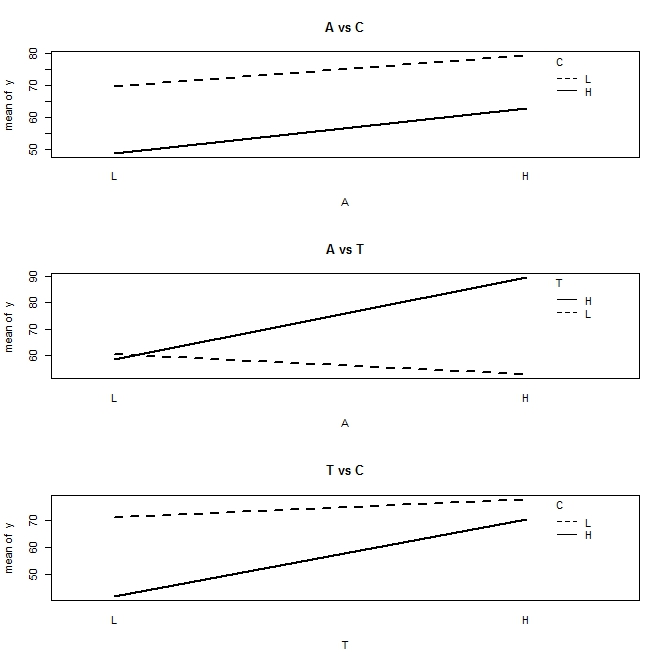
\includegraphics[width=1.1\linewidth]{images/Repeat2017-interactionplots}
\caption{Question 4 Part B : Interaction Plots}
\label{fig:Repeat2017-interactionplots}
\end{figure}








\newpage

\section*{Question 5. (25 marks) Statistical Process Control }

\begin{itemize}



	\item[(a)] (3 Marks) Write a brief description of the Mahalanobis Distance. Illustrate your answer with a sketch.

\item[(b)] A normally distributed quality characteristic is monitored through the use of control charts. These charts have the following parameters. All charts are in control.
\begin{center}
	\begin{tabular}{|c|c|c|c|}
		\hline  & LCL & Centre Line & UCL \\
		\hline $\bar{X}$-Chart & 542 & 550 & 558 \\
		\hline $R$-Chart & 0 & 8.236 & 16.504 \\ \hline
	\end{tabular}
\end{center}

\begin{itemize}
	\item[i] (2 Marks) What sample size is being used for this analysis?
	\item[ii.] (2 Marks) Estimate the standard deviation of this process.
	\item[iii.] (2 Marks) Compute the control limits for the process standard deviation chart (i.e. the s-chart).
\end{itemize}	


\item[(c)]
An automobile assembly plant concerned about quality improvement measured sets of five camshafts on twenty occasions throughout the day. The specifications for the process state that the design specification limits are 600$\pm$3mm.


\begin{itemize}
	\item[(i)] (4 Marks) Determine the \emph{Process Capability Indices} $C_p$ and $C_{pk}$, commenting on the respective values. Use the \texttt{R} code output shown below.
	\item[(ii)] (2 Mark)  Explain why there would be a discrepancy between $C_p$ and $C_{pk}$. Illustrate your answer with sketches.
	\item[(iii)] (1 Mark) Comment on the graphical output of the \emph{Process Capability Analysis}, also presented on the next page.
\end{itemize}


\begin{framed}
	\begin{verbatim}
	Process Capability Analysis
	
	Call:
	process.capability(object = obj,  
	spec.limits = c(597, 603))
	Number of obs = 100          Target = 600
	Center = 599.548         LSL = 597
	StdDev = 0.5846948       USL = 603
	
	Capability indices:
  	   Value   2.5%  97.5%
	Cp    ...
	Cp_l  ...
	Cp_u  ...
	Cp_k  ...
	Cpm   1.353  1.134  1.572
	Exp<LSL 0%   Obs<LSL 0%
	\end{verbatim}
\end{framed}



\begin{center}
	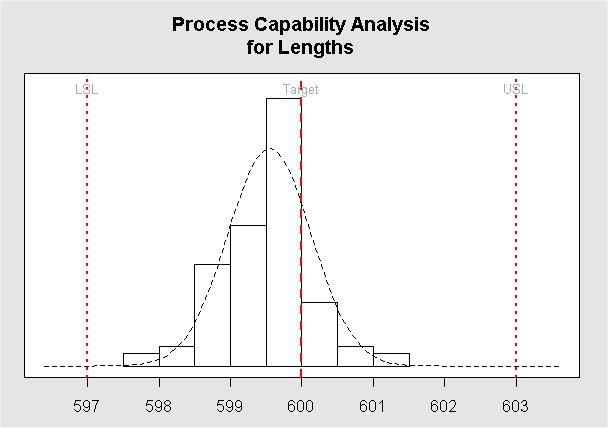
\includegraphics[scale=0.55]{images/ExamQ4hist}
\end{center}

\item[(d)] ($3 \times 3$ Marks) The \textbf{Nelson Rules} are a set of eight decision rules for detecting ``out-of-control" or non-random conditions on control charts. These rules are applied to a control chart on which the magnitude of some variable is plotted against time. The rules are based on the mean value and the standard deviation of the samples.\\

  Discuss any three of these rules, stating their mathematical basis and how they would be used to detect ``out of control" processes. Support your answer with sketch. 


\bigskip 

	\noindent \textit{In your answer, you may make reference to the following properties of the Normal Distribution. Consider the random variable $X$ distributed as
		\[X \sim \mathcal{N}(\mu,\sigma^2)\]
		where $\mu$ is the mean and $\sigma^2$ is the variance of $X$.}
	\begin{itemize}
		\item[$\ast$] $\Pr( \mu - 1\sigma \leq X \leq \mu + 1\sigma ) = 0.6827$
		\item[$\ast$] $\Pr( \mu - 2\sigma \leq X \leq \mu + 2\sigma ) = 0.9545$
		\item[$\ast$] $\Pr( \mu - 3\sigma \leq X \leq \mu + 3\sigma )= 0.9973$
		
	\end{itemize}


\end{itemize}
\section*{Formulas and Tables}

\subsection*{Critical Values for Dixon Q Test}


	{
		\Large
		\begin{center}
			\begin{tabular}{|c|c|c|c|}
				\hline  N  & $\alpha=0.10$  & $\alpha=0.05$  & $\alpha=0.01$  \\ \hline
				3  & 0.941 & 0.97  & 0.994 \\ \hline
				4  & 0.765 & 0.829 & 0.926 \\ \hline
				5  & 0.642 & 0.71  & 0.821 \\ \hline
				6  & 0.56  & 0.625 & 0.74  \\ \hline
				7  & 0.507 & 0.568 & 0.68  \\ \hline
				8  & 0.468 & 0.526 & 0.634 \\ \hline
				9  & 0.437 & 0.493 & 0.598 \\ \hline
				10 & 0.412 & 0.466 & 0.568 \\ \hline
				11 & 0.392 & 0.444 & 0.542 \\ \hline
				12 & 0.376 & 0.426 & 0.522 \\ \hline
				13 & 0.361 & 0.41  & 0.503 \\ \hline
				14 & 0.349 & 0.396 & 0.488 \\ \hline
				15 & 0.338 & 0.384 & 0.475 \\ \hline
				16 & 0.329 & 0.374 & 0.463 \\ \hline
			\end{tabular} 
		\end{center}
	}

\subsection*{Two Way ANOVA}
\begin{multicols}{2}
	
\[MS_A = c \times S^2_r\]

\[MS_B = r \times S^2_c\]
\end{multicols}


\subsection*{Control Limits for Control Charts}

\begin{multicols}{2}
	
\[ \bar{\bar{x}} \pm 3\frac{\bar{s}}{c_4\sqrt{n}}\]

\[ \bar{s} \pm 3\frac{c_5\bar{s}}{c_4}\]

\[\left[ \bar{R}D_3, \bar{R}D_4\right]\]
\end{multicols}
\subsection*{$2^3$ Design: Interaction Effects}

\[ AB = \frac{1}{4n} \left[ abc - bc + ab - b - ac + c - a + (1) \right] \]

\[ AC = \frac{1}{4n} \left[ (1) - a + b - ab -c + ac - bc + abc \right] \]

\[ BC = \frac{1}{4n} \left[ (1) + a - b - ab - c - ac + bc + abc \right] \]

\[ABC = \frac{1}{4n} \left[ abc - bc - ac + c - ab + b +  a - (1) \right] \]

\bigskip


\subsection*{Factorial Design: Sums of Squares}

\[\mbox{Effect} =  \frac{\mbox{Contrast}}{4n}\]

\[\mbox{Sums of Squares} =  \frac{\mbox{(Contrast)}^2}{8n}\]

%------------------------------------------------------------------------ %
\normalsize{
\subsection*{Process Capability Indices}
\begin{multicols}{2}
\[ \hat{C}_p = \frac{\mbox{USL} - \mbox{LSL}}{6s}\]

\[ \hat{C}_{pk} = \mbox{min} \left[\frac{\mbox{USL} - \bar{x}}{3s},\frac{\bar{x} - \mbox{LSL}}{3s} \right] \]

\[ \hat{C}_{pm} = \frac{\mbox{USL} - \mbox{LSL}}{6\sqrt{s^2+(\bar{x}-T)^2}}\]
\end{multicols}
	\newpage
	
	%------------------------------------------------------------------------ %
	\Large{
		\subsection*{Factors for Control Charts}
		\begin{tabular}{|c|c|c|c|c|c|c|}
			\hline
			Sample Size (n) 	&	c4 	&	c5 	&	d2 	&	d3 	&	D3 	&	D4	\\	\hline
			2	&	0.7979	&	0.6028	&	1.128	&	0.853	&	0	&	3.267	\\	
			3	&	0.8862	&	0.4633	&	1.693	&	0.888	&	0	&	2.574	\\	
			4	&	0.9213	&	0.3889	&	2.059	&	0.88	&	0	&	2.282	\\	
			5	&	0.9400	&	0.3412	&	2.326	&	0.864	&	0	&	2.114	\\	
			6	&	0.9515	&	0.3076	&	2.534	&	0.848	&	0	&	2.004	\\	
			7	&	0.9594	&	0.282	&	2.704	&	0.833	&	0.076	&	1.924	\\	
			8	&	0.9650	&	0.2622	&	2.847	&	0.82	&	0.136	&	1.864	\\	
			9	&	0.9693	&	0.2459	&	2.970	&	0.808	&	0.184	&	1.816	\\	
			10	&	0.9727	&	0.2321	&	3.078	&	0.797	&	0.223	&	1.777	\\	
			11	&	0.9754	&	0.2204	&	3.173	&	0.787	&	0.256	&	1.744	\\	
			12	&	0.9776	&	0.2105	&	3.258	&	0.778	&	0.283	&	1.717	\\	
			13	&	0.9794	&	0.2019	&	3.336	&	0.770	&	0.307	&	1.693	\\	
			14	&	0.9810	&	0.1940	&	3.407	&	0.763	&	0.328	&	1.672	\\	
			15	&	0.9823	&	0.1873	&	3.472	&	0.756	&	0.347	&	1.653	\\	
			16	&	0.9835	&	0.1809	&	3.532	&	0.750	&	0.363	&	1.637	\\
			17	&	0.9845	&	0.1754	&	3.588	&	0.744	&	0.378	&	1.622	\\
			18	&	0.9854	&	0.1703	&	3.64	&	0.739	&	0.391	&	1.608	\\
			19	&	0.9862	&	0.1656	&	3.689	&	0.734	&	0.403	&	1.597	\\
			20	&	0.9869	&	0.1613	&	3.735	&	0.729	&	0.415	&	1.585	\\
			21	&	0.9876	&	0.1570	&	3.778	&	0.724	&	0.425	&	1.575	\\
			22	&	0.9882	&	0.1532	&	3.819	&	0.720	&	0.434	&	1.566	\\
			23	&	0.9887	&	0.1499	&	3.858	&	0.716	&	0.443	&	1.557	\\
			24	&	0.9892	&	0.1466	&	3.895	&	0.712	&	0.451	&	1.548	\\
			25	&	0.9896	&	0.1438	&	3.931	&	0.708	&	0.459	&	1.541	\\
			\hline
		\end{tabular}
	} % End Large Font
	
\end{document}

Outliers
Boxplots Outliers ( Upper Fence Lower Fence)
Dixon Q-Test
%----------------------------------%
Chi Square 12 Marks
%=====================================================




\section{Question 6- Standby Questions}



\subsubsection*{Question 3 Part C (7 Marks)}
Six analysts each made seven determinations of the paracetamol content of the same batch of tablets.
The results are shown below. There are 42 determinations in total. 
%The mean determination for each analysts is also tabulated. \\


%Analyst= structure(c(1L, 2L, 3L, 4L, 5L, 6L, 1L, 2L, 3L, 4L, 5L, 6L, 1L,
%2L, 3L, 4L, 5L, 6L, 1L, 2L, 3L, 4L, 5L, 6L, 1L, 2L, 3L, 4L, 5L,
%6L, 1L, 2L, 3L, 4L, 5L, 6L, 1L, 2L, 3L, 4L, 5L, 6L), .Label = c("A",
%"B", "C", "D", "E", "F"), class = "factor")

%Determinations= c(84.32, 84.24, 84.29, 84.14, 84.5, 84.7, 84.61, 84.13, 84.28,
%84.48, 83.91, 84.36, 84.64, 84, 84.4, 84.27, 84.11, 84.61, 84.62,
%84.02, 84.63, 84.22, 83.99, 84.15, 84.51, 84.25, 84.4, 84.22,
%83.88, 84.17, 84.63, 84.41, 84.68, 84.02, 84.49, 84.11, 84.51,
%84.3, 84.36, 84.33, 84.06, 83.81)

\begin{center}
	\begin{tabular}{|c|ccccccc|}
		\hline
		Analyst	& Content		&		&		&		&		&		&		 \\ \hline
		A	&	84.32	&	84.61	&	84.64	&	84.62	&	84.51	&	84.63	&	84.51	 \\
		B	&	84.24	&	84.13	&	84.00	&	84.02	&	84.25	&	84.41	&	84.30	 \\
		C	&	84.29	&	84.28	&	84.40	&	84.63	&	84.40	&	84.68	&	84.36	 \\
		D	&	84.14	&	84.48	&	84.27	&	84.22	&	84.22	&	84.02	&	84.33	 \\
		E	&	84.50	&	83.91	&	84.11	&	83.99	&	83.88	&	84.49	&	84.06	 \\
		F	&	84.70	&	84.36	&	84.61	&	84.15	&	84.17	&	84.11	&	83.81	 \\
		\hline
	\end{tabular}
\end{center}
\bigskip
The following \texttt{R} output has been produced as a result of analysis of these data:

%Experiment=data.frame(Determinations, Analyst)
%Model=aov(Determinations~Analyst)
%summary(Model)
\begin{framed}
	\begin{verbatim}
	Analysis of Variance Table
	
	Df   Sum Sq   Mean Sq   F value    Pr(>F)
	Analyst        5   0.8611   0.17222     4.236   0.00394 **
	Residuals     36   1.4635   0.04065
	---
	Signif. codes:  0 ‘***’ 0.001 ‘**’ 0.01 ‘*’ 0.05 ‘.’ 0.1 ‘ ’ 1
	\end{verbatim}
\end{framed}

%\subsubsection*{Vegetables (ONE WAY ANOVA 4505)}
%
%(c) The following data give the recovery of bromide from spiked samples of vegetable matter, measured using a gas-liquid chromatographic method. The same amount of bromide was added to each specimen. 
%
%The units for all measurements are  mg g-1
%
%\begin{center}
%	\begin{tabular}{|c|c|c|c|}
%		Tomato: & $\{777 790 759 790 770 758 764\}$ & 774 & 142.6667
%		\\ \hline
%		
%		Cucumber: & $\{782 773 778 765 789 797 782\}$ & 781 &  106\\ \hline
%		
%		Asparagus : & $\{786 783 781 785 789 797 782 \}$& 785 & \\ \hline
%	\end{tabular} 
%\end{center}


%-------------------------------------------------------------------------------
%y<-c(777, 789, 769, 790, 770, 759, 764, 782, 774, 778, 765, 789, 
%797, 782, 785, 783, 782, 785, 787, 791, 782)
%
%
%
%T<-y[1:7];C<-y[8:14];A<-y[15:21];
%mean(T);mean(C);mean(A);
%
%-------------------------------------------------------------------------------
%-------------------------------------------------------------------------------

%
%
%\begin{itemize}
%	\item[(i)](3 Marks) Compute the Between Groups Sum of Squares, \textit{Show your workings}
%	\item[(ii)](3 Marks) Compute the Within Groups Sum of Squares, \textit{Show your workings}
%	\item[(iii)](2 Marks) Compute the Total Sum of Squares,\textit{ show your workings}
%	\item[(iv)] (2 Marks) Degrees of Fredom columns
%	\item[(v)] (1 Marks) Mean Square
%	\item[(vi)] (1 Marks) F test Statistics
%\end{itemize}
%\begin{tabular}{|c|c|c|c|c|c|}
%	\hline Source & DF & SS & MS & F & p-value \\ 
%	\hline Between &  &  &  &  &  \\ 
%	\hline Within &  &  &  &  &  \\ 
%	\hline Total &  &  &  &  &  \\ 
%	\hline 
%\end{tabular} 
%\begin{framed}
%	\begin{verbatim}
%	> bartlett.test(y~group)
%	
%	Bartlett test of homogeneity of variances
%	
%	data:  y by group
%	Bartlett's K-squared = 7.9063, df = 2, p-value = 0.01919
%	
%	\end{verbatim}
%\end{framed}

%====================================================================== %


%Experiment=data.frame(Determinations, Analyst)
%Model=aov(Determinations~Analyst)
%summary(Model)

%Analysis of Variance Table
%
%            Df Sum Sq Mean Sq F value  Pr(>F)
%Analyst      5 0.8611 0.17222   4.236 0.00394 **
%Residuals   36 1.4635 0.04065
%---
%Signif. codes:  0 ‘***’ 0.001 ‘**’ 0.01 ‘*’ 0.05 ‘.’ 0.1 ‘ ’ 1

\begin{center}
	\texttt{
		\begin{tabular}{|cc|c|c|c|c|c|}
			\hline
			% after \\: \hline or \cline{col1-col2} \cline{col3-col4} ...
			&&		&		&		&		&		\\
			Response: Y        	&&	Df  	&	Sum Sq 	&	Mean Sq 	&	F value    	&	$Pr(>F)$    	\\
			&&	\phantom{make}	&		&		&		&		\\\hline \hline
			&&		&	\phantom{make}	&		&		&		\\
			Analyst 	&&	\textbf{?}	&	\textbf{?}	&	\textbf{?}	&	\textbf{?}	&	0.00394 **	\\
			&&		&		&		&		&		\\ \hline
			&&		&		&		&		&		\\
			Residuals	&&	\textbf{?}	&	\textbf{?}	&	0.04065	&	&		\\
			&&		&		&		&		&		\\ \hline
			&&		&		&		&		&		\\
			Total	&&	\textbf{?}	&	2.3246	&		&		&		\\
			&&		&		&		&		&		\\ \hline
		\end{tabular}
	}
\end{center}
\begin{itemize}
	\item[(i.)] (6 Marks) Complete the ANOVA table in your answer sheet, replacing the "?" entries with the correct values.\textit{\\ (You are not required to carry out a hypothesis test.)}
	%	\item[ii.] (2 marks) What hypothesis is being considered by this procedure.
	
\end{itemize}
\newpage




\section{R Code for Part 3}
\begin{verbatim}
ALL <- c(84.32, 84.51, 84.63, 84.61, 84.64, 84.51, 84.62, 84.24, 84.25, 
84.41, 84.13, 84, 84.3, 84.02, 84.29, 84.4, 84.68, 84.28, 84.4, 
84.36, 84.63, 84.14, 84.22, 84.02, 84.48, 84.27, 84.33, 84.22, 
84.5, 83.88, 84.49, 83.91, 84.11, 84.06, 83.99, 84.7, 84.17, 
84.11, 84.36, 84.61, 83.81, 84.15)

\end{verbatim}
%==================================================%
library(xtable)

nu1 <- 2:10
nu2 <- c(5:15,18,21,24,27,30)

L1 <- length(nu1)
L2 <- length(nu2)
CVs <- matrix(ncol=L1,nrow=L2)


for( i in 1:L2){
	for( j in 1:L1){ 
		CVs[i,j] <- round( qf(0.95,i,j),3)
	}
	
}

colnames(CVs)<- nu1

rownames(CVs)<- nu2

xtable(CVs) 

%======================================================================= %
Dixon

chi Square

Normal

One Way ANOVA

Two Way ANOVA interactions

Test Normality

SPC definitions





min=23
max=89
range=65
gap=31
TS =31/65 = 0.47692
CV =0.396 (5\%)
Reject Ho


